\documentclass[oneside,final,14pt,a4paper]{extreport}

\usepackage{tempora}

\usepackage{vmargin}
\setpapersize{A4}
\setmarginsrb{2.5cm}{2cm}{2cm}{2cm}{0pt}{10mm}{0pt}{13mm}
\usepackage{setspace}
\setstretch{1.5}
\usepackage{indentfirst}
\parindent=1.25cm

\usepackage[T1,T2A]{fontenc}
\usepackage[utf8]{inputenc}
\usepackage[english,russian]{babel}

\usepackage[backend=biber,style=ieee,sorting=none]{biblatex}
\addbibresource{ref.bib}

\usepackage{amsmath,amsfonts}
\usepackage{enumitem}
\usepackage{hyperref}
\hypersetup{colorlinks=true, linkcolor=black, citecolor=black, urlcolor=black}
\usepackage{pdfpages}

\setlength{\parindent}{1.25cm}

\begin{document}

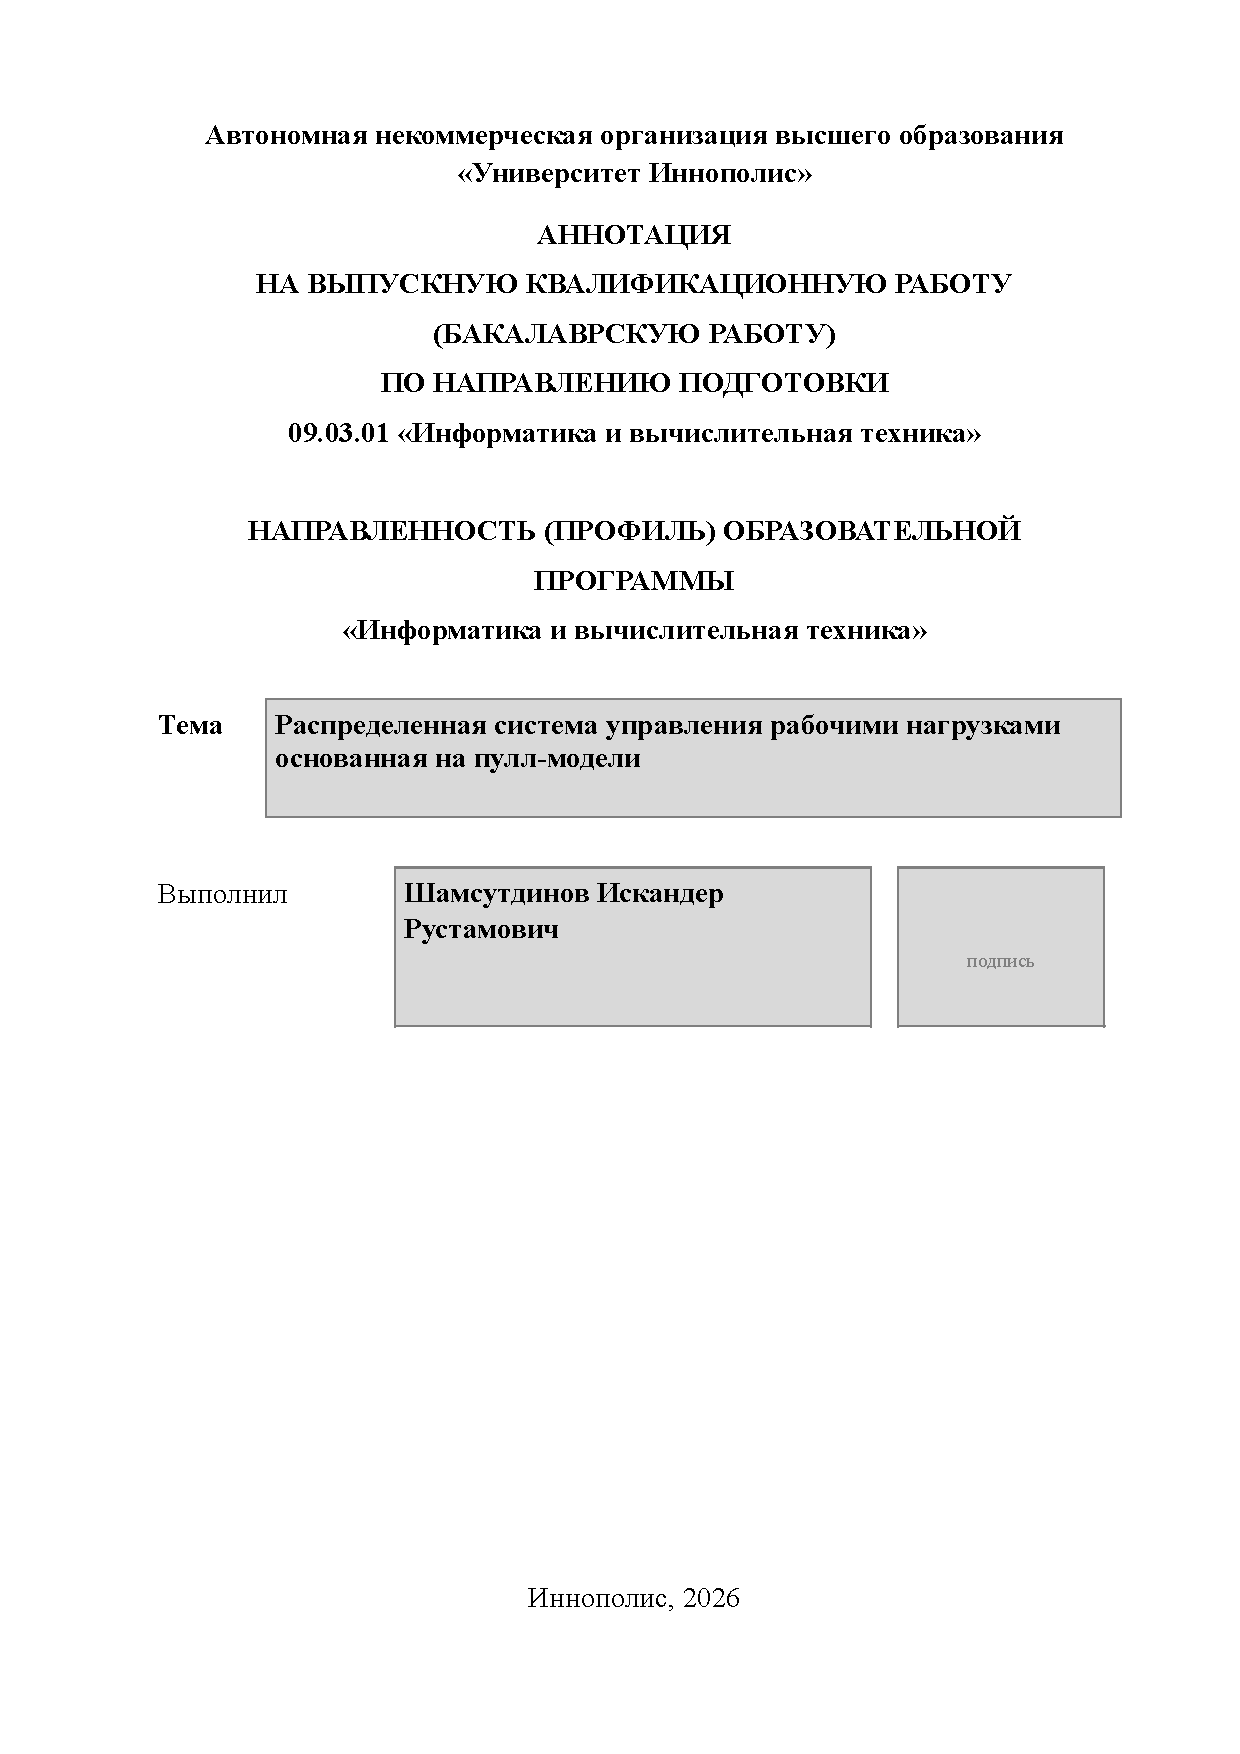
\includepdf[pages=-, offset=70 -80]{annotation_title.pdf}

\tableofcontents
\newpage

\chapter*{Введение}
\addcontentsline{toc}{chapter}{Введение}

\section*{Актуальность темы исследования}

Kubernetes~\cite{k8s_docs} и HashiCorp Nomad~\cite{nomad_docs} стали стандартом
для запуска контейнеров в распределённой среде, однако за это приходится платить
ресурсами и операционной нагрузкой на сопровождение. Даже у минимального
отказоустойчивого кластера Kubernetes управляющий слой занимает порядка 13 ядер и
18{,}5~ГБ памяти, и под сами приложения из этих ресурсов остаётся меньше 8~\%. При
дальнейшем масштабировании кластера эти затраты распределяются на множество узлов
и в относительном выражении становятся незначительными, однако для небольших
компаний с ограниченной инфраструктурой они ощутимы, поскольку фиксированная
стоимость управляющего слоя приходится на малое число рабочих узлов. Ключевую же
роль играет то, что планирование остаётся за управляющим слоем: его
планировщик решает, на какой узел отправить нагрузку, и лишь после этого
конфигурация доставляется на узел по pull-схеме. Такая централизация делает
планировщик единой точкой отказа и узким местом, а сопровождение системы обычно
требует отдельной команды инженеров.

Предлагаемая альтернатива переносит планирование на узлы: управляющий слой вообще
не принимает решений о размещении, а узлы сами обращаются к нему, забирают
свободные нагрузки и захватывают на них аренду (lease), подтверждая, что нагрузка
теперь закреплена за ними~\cite{hiku2025pull, gray1989leases}.
Координацию при этом берёт на себя реляционная база данных, а не отдельный
протокол консенсуса; такой выбор сознательно отдаёт предпочтение доступности и
устойчивости к разрывам сети перед строгой
согласованностью~\cite{brewer2012cap, decandia2007dynamo}. Оценить
жизнеспособность такого подхода на практике можно только на работающем прототипе,
проверенном на реальной распределённой инфраструктуре.

\section*{Цель работы}

Спроектировать и реализовать прототип системы управления распределёнными
нагрузками на основе pull-модели и проверить на практике, удаётся ли при этом
надёжно планировать нагрузки и восстанавливаться после отказов, расходуя на
управляющий слой заметно меньше ресурсов, чем существующие оркестраторы.

\section*{Задачи исследования}

\begin{enumerate}[left=0pt]
\item Изучить Kubernetes и Nomad, оценить их эксплуатационные и ресурсные
издержки и на этой основе сформулировать требования к прототипу.
\item Спроектировать децентрализованную архитектуру: управляющий слой без
собственного состояния, хранение в PostgreSQL и захват нагрузок через механизм
аренды.
\item Реализовать четыре компонента: управляющий слой, агент, ингресс-прокси
(Edge) и консольную утилиту \texttt{mctl}.
\item Измерить на реальной инфраструктуре время планирования (SLO) и время
восстановления (RTO) в пяти сценариях, по 100 прогонов в каждом.
\item Сравнить ресурсы, которые требует управляющий слой прототипа, с Kubernetes
и Nomad.
\end{enumerate}

\section*{Объект и предмет исследования}

Объектом исследования выступает распределённая система оркестрации
кратковременных нагрузок. Предметом является pull-модель координации, при которой
агенты сами опрашивают управляющий слой без состояния и захватывают эксклюзивную
аренду через реляционную базу данных. Работа построена по методологии Design
Science Research~\cite{dresch2014design}, в рамках которой выявление проблемы,
проектирование и оценка артефакта выполняются итеративно.

\section*{Научная новизна}

\begin{enumerate}[left=0pt]
\item Предложен прототип оркестратора, в котором управляющий слой не хранит
состояния, осуществляет координацию через PostgreSQL, а отказоустойчивость
обеспечивается одним лишь истечением аренды, без протоколов консенсуса и
механизмов heartbeat.
\item Показано, что восстановление работает надёжно: средний RTO составил
47{,}8~с (95~\% ДИ [45{,}8; 49{,}8]), все 100 прогонов завершились успешно, и
система уложилась в целевые 90~с.
\item Измерена экономия ресурсов: в сопоставимой отказоустойчивой конфигурации
управляющему слою достаточно 1{,}75 ядра и 3{,}25~ГБ против 13 ядер и 18{,}5~ГБ у
Kubernetes.
\item Выявлены издержки совмещения нагрузок на одном узле: два контейнера на одном
узле планируются на 76~\% дольше, чем разнесённые по разным узлам (31{,}5~с против
17{,}9~с).
\end{enumerate}

\chapter*{Краткое описание основной части работы}
\addcontentsline{toc}{chapter}{Краткое описание основной части работы}

\textbf{Глава 1. Введение.} Обозначает проблему, а именно высокую стоимость и
уязвимость push-планирования в существующих оркестраторах, и ставит два
исследовательских вопроса: можно ли с помощью pull-модели снизить издержки, не
теряя в отказоустойчивости, и на какие компромиссы при этом приходится идти. Здесь
же изложена методология Design Science Research.

\textbf{Глава 2. Обзор литературы.} Обобщает работы по оркестрации и
децентрализованному планированию: от Borg~\cite{verma2015borg} и Omega до
распределённых Sparrow и Apollo; pull-планирование в бессерверных
средах~\cite{hiku2025pull}; теорему CAP и архитектуры с приоритетом
доступности~\cite{brewer2012cap, decandia2007dynamo}; аренду как примитив
координации~\cite{gray1989leases}; облегчённую оркестрацию для
периферийных сред~\cite{cilic2023edgeeval}.

\textbf{Глава 3. Выявление проблемы.} На примере B2B-сервиса аутентификации
показано, во что обходится отказ узла: без оркестрации теряется около 3000
запросов, тогда как оркестрация сокращает RTO до 90~с. Разбираются Kubernetes и
Nomad, из анализа выводятся три функциональных и четыре нефункциональных
требования, среди них RTO не более 90~с и mTLS на всех каналах между
компонентами.

\textbf{Глава 4. Реализация.} Объясняет, почему выбрана pull-модель, и описывает
деление системы на управляющий слой и слой данных. Управляющий слой не хранит
состояния, опирается на PostgreSQL и взаимодействует по REST поверх HTTPS с mTLS.
Шесть технических сценариев иллюстрируют полный цикл работы с нагрузкой: создание,
опрос агентом, захват аренды, жизненный цикл контейнера, истечение аренды и
маршрутизацию через Edge. Исходный код опубликован в открытом доступе.

\textbf{Глава 5. Оценка.} Описывает стенд в Selectel (3 узла по 2 ядра и 4~ГБ),
пять сценариев по 100 прогонов и метрики SLO и RTO. Приводит результаты, критерий
Манна\,–\,Уитни (p~<~0{,}001), сравнение по ресурсам и пять угроз достоверности.

\textbf{Глава 6. Заключение.} Подводит итоги по обоим исследовательским вопросам,
называет сильные стороны решения, его ограничения и дальнейшие направления.

\chapter*{Заключение}
\addcontentsline{toc}{chapter}{Заключение}

Прототип на pull-модели планирует нагрузки предсказуемо: одиночную нагрузку он
запускает в среднем за 14{,}2~с (95~\% ДИ [13{,}8; 14{,}6]), пару на разных узлах
за 17{,}9~с, две нагрузки на одном узле за 31{,}5~с. После отказа узла система
восстанавливается за 47{,}8~с в среднем (95~\% ДИ [45{,}8; 49{,}8];
P95~=~59{,}3~с) и во всех 100 прогонах укладывается в целевые 90~с. Критерий
Манна\,–\,Уитни подтверждает, что накладные расходы значимы и при распределённом,
и при одноузловом планировании (p~<~0{,}001). За 700 размещений нагрузок не
случилось ни одного конфликта аренды и ни одного двойного захвата.

Управляющему слою достаточно 0{,}5 ядра и 1~ГБ памяти, а в отказоустойчивой
конфигурации требуется 1{,}75 ядра и 3{,}25~ГБ; это в разы меньше Kubernetes
(13 ядер, 18{,}5~ГБ) и ниже Nomad. Экономия достигается тем, что управляющий слой
не хранит состояния: его реплики взаимозаменяемы, им не нужны ни консенсус, ни
выбор лидера, и предел масштабирования упирается в пропускную способность
PostgreSQL, а не в саму модель оркестрации.

Простота решения сопряжена с рядом ограничений. Планировщик работает по принципу
«первым пришёл, первым обслужен», а 30-секундный таймаут аренды задаёт нижнюю
границу скорости обнаружения отказа (значение настраивается). Экспериментальная
проверка охватила лишь два агента и две нагрузки на узел, минимальные образы
контейнеров и один сетевой регион. В дальнейшем целесообразно проверить систему
на десятках агентов и сотнях нагрузок, выполнить длительные прогоны для поиска
утечек и добавить правила выбора узлов, поэтапные обновления (rolling updates),
абстракцию реплик и телеметрию.

\printbibliography[heading=bibintoc, title={Список использованных источников}]

\end{document}
